\chapter{Infrastructure}

\justify{}
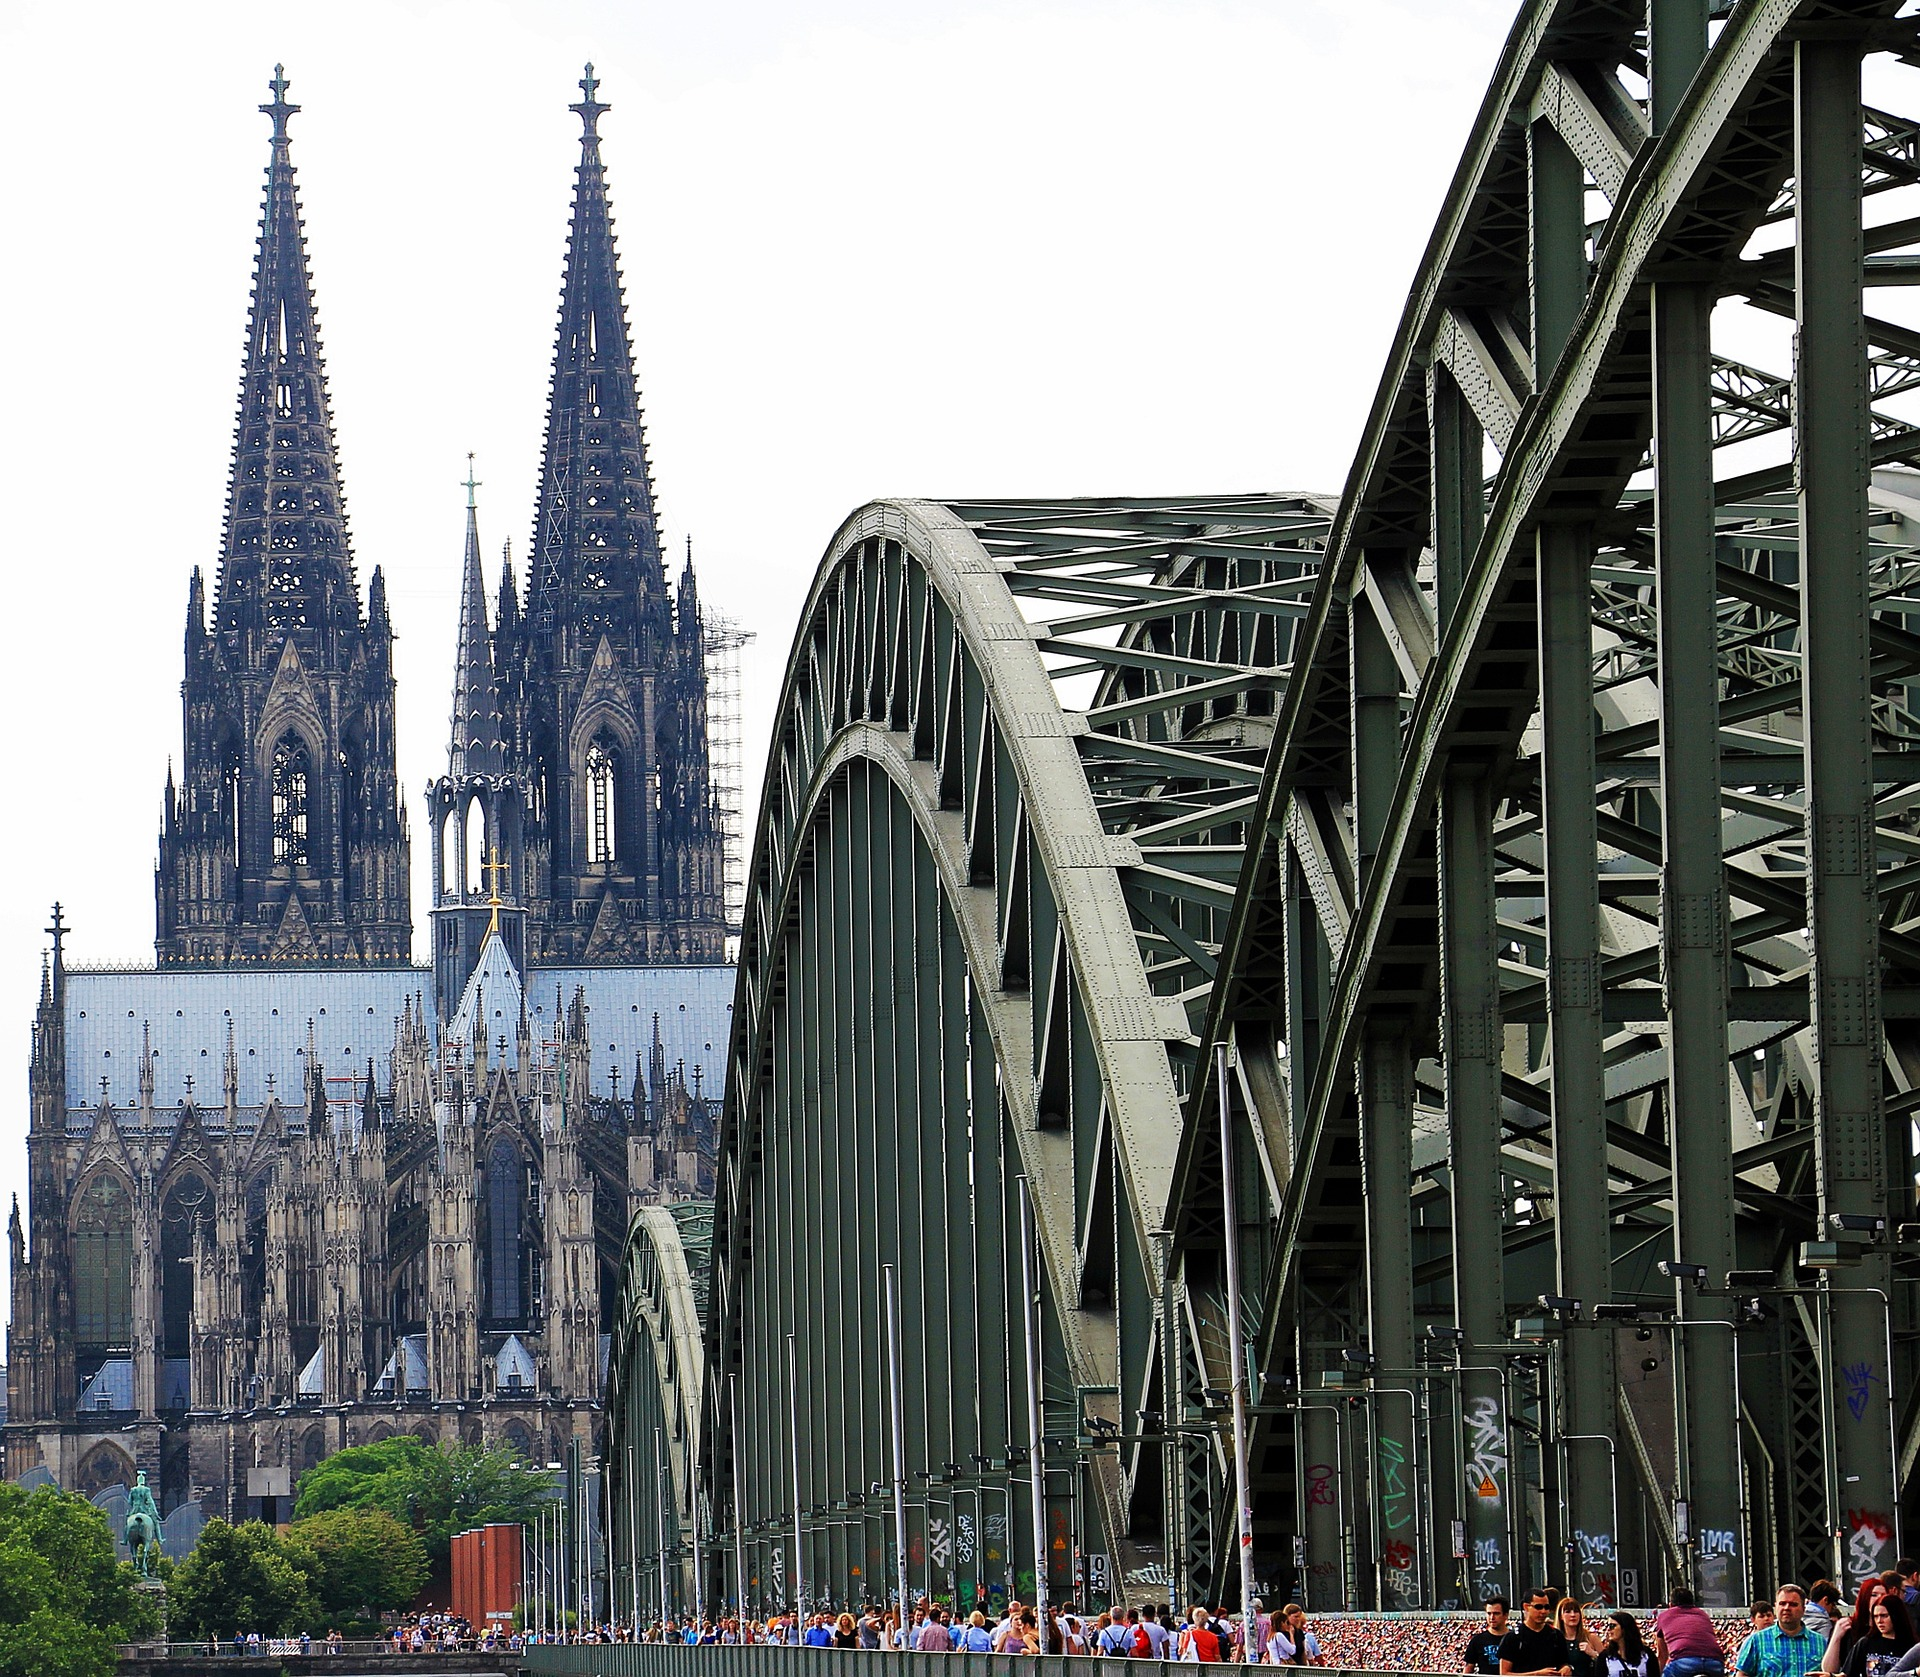
\includegraphics{images/cologne-cathedral-1507854_1920.jpg}

\justify{}
Software Infrastructure and Platforms are the foundations upon which our
scripts, code, and projects are founded. Infrastructure comprises the
base upon which our containers rest, and the connectivity that allows us
to communicate with them and them with each other.

\justify{}
This chapter details our ability to quickly and uniformly stand up and
tear down virtual domains and networks to connect our containers and
route their workloads. We will look at some popular cloud computing
providers to prepare to explore ways we can leverage them to our
benefit.

\justify{}
A Public Cloud Provider is a company that offers to host our containerized
projects and virtual infrastructure so we don't have to do it ourselves.

\justify{}
The virtual resources we subscribe to will be distributed across cloud
provider hardware in data centers around the world with very little
oversight or interaction from us. For example, we can choose a Region of
the world for our server instance to exist in, but we don't need to
worry about which machine or rack it's in, or even where the data center
is located.

\section{Amazon Web Services (AWS)}

\justify{}
Consider\fig{aws} which illustrates the connectivity of a basic
project using Amazon Web Services (AWS)\index{Amazon Web Services}.

\begin{figure}
  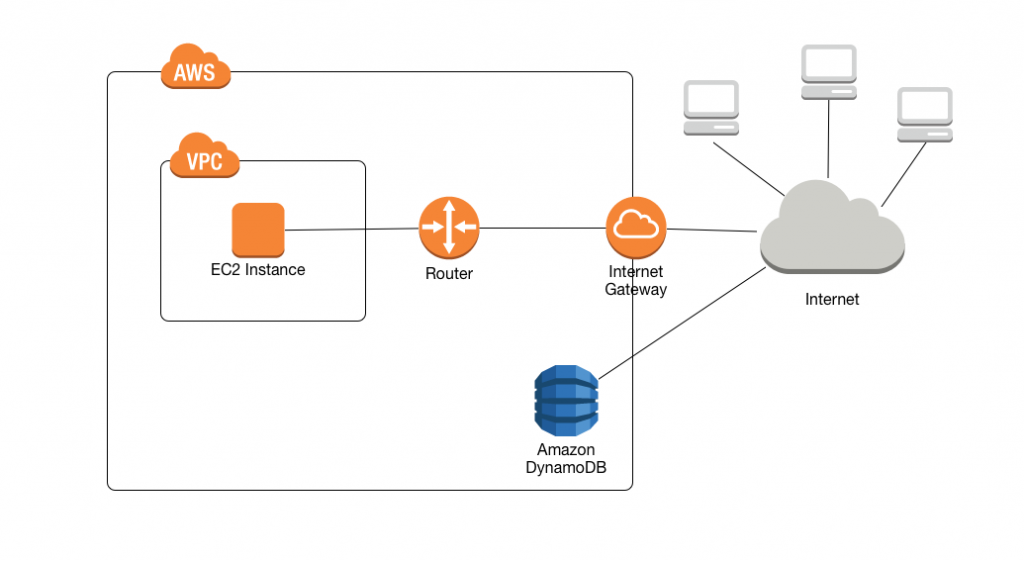
\includegraphics[scale=0.45]{images/ddb-no-vpc-endpoint-1024x561.png}
  \caption{A simple Public Cloud configuration using AWS as a provider.}
\label{aws}
\end{figure}

\subsection{Getting Set up in AWS}

\justify{}
One of the very first things you should do (after creating an account,
that is) is to configure mutli-factor authentication (MFA)\index{multi-factor authentication}.

\justify{}
Amazon's AWS is one of the more prevalent cloud providers in terms of
popularity and simultaneously mature and ever-expanding feature set.

\subsection{Credentials}
\justify{}
Amazon Web Services (AWS) credentials are stored in a hidden directory
in your home directory called ``.aws''. The file
\textasciitilde{}/.aws/credentials should be modified to contain your
AWS access\_id and secret\_key as seen below.

\begin{mybox}{\thetcbcounter: ~/.aws/credentials}
  \lstinputlisting{code/09-infra/aws-creds.txt}
\end{mybox}

\justify{}
Do not share this file with other people. Do not check this file into
your GitHub repositories under any circumstances.

\section{Google Cloud Platform (GCP)}

\justify{}
Google Cloud Platform (GCP) is a suite of cloud computing services that
runs on the same infrastructure that Google uses internally for its
end-user products. If the
resources we allocate on GCP were a pyramid, the apex of that pyramid
would be a ``project''. A project is made up of the settings, permissions,
and other metadata that describe your application.

single: Google Cloud Platform single: GCP

\justify{}
One of the very first things you should do (after creating an account,
that is) is to configure two-factor authentication\index{two-factor authentication}
(2FA)\index{2FA}.

\justify{}
At this point you are ready to install the gcloud\index{gcloud} software development
kit (SDK) on your local machine.

\subsection{Credentials}

\justify{}
Once the gcloud SDK is installed, you are ready to set up local
credentials that allow interaction between your machine and the GCP
application programming interface (API). In other words, Google hosts a
server that you can exchange commands with to configure your GCP
projects from your local CLI.

\justify{}
GCP credentials are stored in the directory
\textasciitilde{}/.config/gcloud as a JSON file. Do not share this file
with other people. Do not check this file into your GitHub repositories
under any circumstances.

\clearpage
\subsection{Directory Structure}

\justify{}
Relevant folders and files related to our build pipeline are shown
below. The users home directory and workspace subdirectory is implied
and removed from the diagram for clarity.

\begin{figure}[!htb]
  
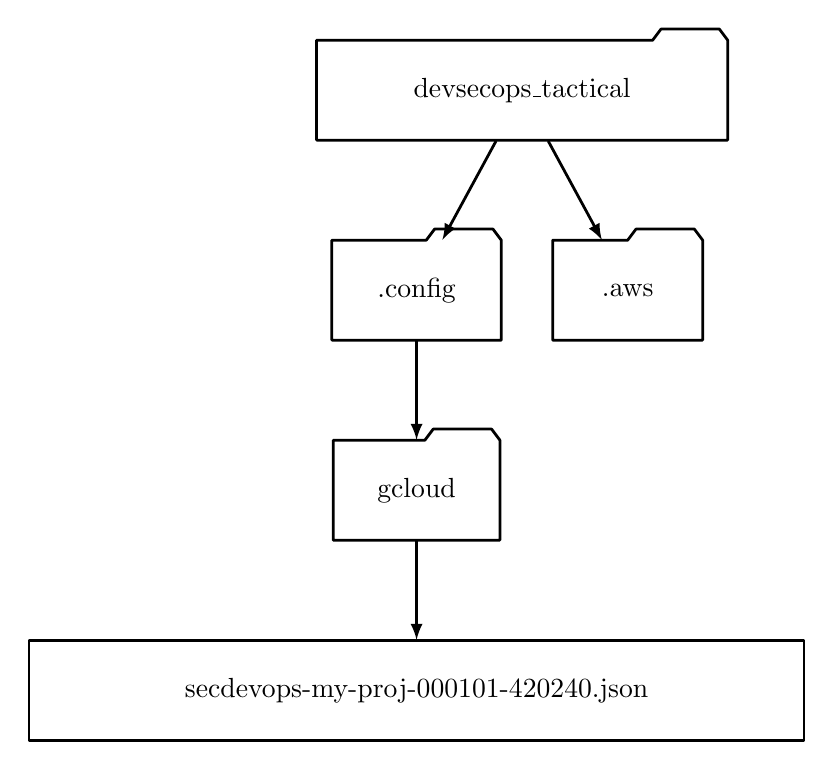
\begin{tikzpicture}[>=latex,line join=bevel,]
  \pgfsetlinewidth{1bp}
%%
\pgfsetcolor{black}
  % Edge: framework -> dotcfg
  \draw [->] (168.11bp,215.7bp) .. controls (163.74bp,207.64bp) and (158.44bp,197.89bp)  .. (148.79bp,180.1bp);
  % Edge: framework -> aws
  \draw [->] (186.89bp,215.7bp) .. controls (191.26bp,207.64bp) and (196.56bp,197.89bp)  .. (206.21bp,180.1bp);
  % Edge: dotcfg -> gcloud
  \draw [->] (139.5bp,143.7bp) .. controls (139.5bp,135.98bp) and (139.5bp,126.71bp)  .. (139.5bp,108.1bp);
  % Edge: gcloud -> sdo
  \draw [->] (139.5bp,71.697bp) .. controls (139.5bp,63.983bp) and (139.5bp,54.712bp)  .. (139.5bp,36.104bp);
  % Node: framework
\begin{scope}
  \definecolor{strokecol}{rgb}{0.0,0.0,0.0};
  \pgfsetstrokecolor{strokecol}
  \draw (251.5bp,252.0bp) -- (248.5bp,256.0bp) -- (227.5bp,256.0bp) -- (224.5bp,252.0bp) -- (103.5bp,252.0bp) -- (103.5bp,216.0bp) -- (251.5bp,216.0bp) -- cycle;
  \draw (177.5bp,234.0bp) node {devsecops\_tactical};
\end{scope}
  % Node: dotcfg
\begin{scope}
  \definecolor{strokecol}{rgb}{0.0,0.0,0.0};
  \pgfsetstrokecolor{strokecol}
  \draw (170.0bp,180.0bp) -- (167.0bp,184.0bp) -- (146.0bp,184.0bp) -- (143.0bp,180.0bp) -- (109.0bp,180.0bp) -- (109.0bp,144.0bp) -- (170.0bp,144.0bp) -- cycle;
  \draw (139.5bp,162.0bp) node {.config};
\end{scope}
  % Node: aws
\begin{scope}
  \definecolor{strokecol}{rgb}{0.0,0.0,0.0};
  \pgfsetstrokecolor{strokecol}
  \draw (242.5bp,180.0bp) -- (239.5bp,184.0bp) -- (218.5bp,184.0bp) -- (215.5bp,180.0bp) -- (188.5bp,180.0bp) -- (188.5bp,144.0bp) -- (242.5bp,144.0bp) -- cycle;
  \draw (215.5bp,162.0bp) node {.aws};
\end{scope}
  % Node: gcloud
\begin{scope}
  \definecolor{strokecol}{rgb}{0.0,0.0,0.0};
  \pgfsetstrokecolor{strokecol}
  \draw (169.5bp,108.0bp) -- (166.5bp,112.0bp) -- (145.5bp,112.0bp) -- (142.5bp,108.0bp) -- (109.5bp,108.0bp) -- (109.5bp,72.0bp) -- (169.5bp,72.0bp) -- cycle;
  \draw (139.5bp,90.0bp) node {gcloud};
\end{scope}
  % Node: sdo
\begin{scope}
  \definecolor{strokecol}{rgb}{0.0,0.0,0.0};
  \pgfsetstrokecolor{strokecol}
  \draw (279.0bp,36.0bp) -- (0.0bp,36.0bp) -- (0.0bp,0.0bp) -- (279.0bp,0.0bp) -- cycle;
  \draw (139.5bp,18.0bp) node {secdevops-my-proj-000101-420240.json};
\end{scope}
%
\end{tikzpicture}


  \caption{IaC related files and folders.}
\label{infra}
\end{figure}
